\chapter{Soft-Wall Model of AdS/QCD
\label{sec:Soft-Wall-Model}}
\begin{flushright}
\emph{Ad astra per alas porci}. \\
To the stars on the wings of a pig. \\
--Motto on John Steinbeck's personal stamp
\end{flushright}

In this chapter, we provide detail on previous work on the soft-wall AdS/QCD model.
We present the set-up of the background metric and the fields that must be included in simplest version of the soft-wall model.
The method for modeling the chiral symmetry breaking of QCD is discussed.
The Euler-Lagrange equations for the gauge fields are derived, and the eigenvalue equations for the masses of the meson excited states are presented.

We also describe work done to modify this soft-wall model to capture the correct form of chiral symmetry breaking by adding additional terms to the action.
The changes to the meson equations of motion due to these additional terms are presented.

Finally, we present work on the pseudoscalar sector of the modified soft-wall model, contributed to by the author. 
Two alternative representations for the pseudoscalar field are presented and shown to be equivalent.
We then calculate the meson spectrum for the pions and show that this model satisfies the Gell-Mann--Oakes--Renner relation.

\section{Minimal Soft-Wall Model}
The soft-wall model of AdS/QCD was introduced by Karch, \emph{et al} \cite{karch-katz-son-adsqcd} and studied further by \cite{karch-dilaton-sign,Evans:2006ea,Grigoryan:2007my,kwee-lebed-pion,Cherman2009,colangelo2008,Huang:2007fv}.
This work showed that the behavior of highly-excited mesons is controlled by the infrared behavior of the AdS/CFT dual theory. 
They argued that the simple cut-off of the hard-wall model should be replaced with a field known as the \emph{dilaton} whose IR behavior would act as a smooth cut-off to the AdS space.
In this section, we describe the set-up and field content of such a simple model and compare the resulting behavior to that of a hard-wall model.

\subsection{Metric and Field Content}
The gravitational dual theory exists in  five-dimensional anti-de Sitter space, with a metric given by
\be
ds^{2}=g_{MN}dx^M dx^N=a^{2}(z)(\eta_{\mu\nu}dx^{\mu}dx^{\nu}+dz^{2}),
\ee
where $a(z)=L/z$ is the warp factor and $L$ is the curvature radius of the anti-de Sitter space. 
It is often convenient to work in units where the curvature radius is unity.
The Minkowski metric is given by
\be
\eta_{\mu\nu}= \left( \begin{array}{cccc} 
 -1 & 0 & 0 & 0\\
  0 & 1 & 0 & 0\\
  0 & 0 & 1 & 0\\
  0 & 0 & 0 & 1
\end{array} \right).
\ee
The coordinate $z$ has a range $0 < z < \infty$.

The bulk coordinate $z$ is associated with inverse energy scales, with the ultraviolet limit of QCD represented by fields at $z\rightarrow0$ \cite{kwee-lebed-pion}. 
The AdS/CFT dictionary \cite{maldacena,klebanov-witten} states that each operator $\mathcal{O}(x)$ in the 4D conformal field theory is associated with a bulk field $\psi(x,z)$. 
The values of the bulk fields at the UV boundary act as sources for the corresponding
4D currents. 
Global symmetries of the 4D field theory become gauged symmetries for the bulk fields. 

The generating functional of gauge-invariant operators of the gauge theory is dual to the minimum of the supergravity action. 
On the boundary, the supergravity fields must coincide with the sources of the gauge theory \cite{Gubser:1998bc,Erdmenger:2007cm}. 
That is, 
\be
\left\langle \exp\left[\int_{\partial AdS} d^{4}x\,\phi^{0}(\vec{x})\mathcal{O}(\vec{x)}\right]\right\rangle_{{\rm CFT}}  =  \left. \exp \left[i S_{{\rm SUGRA}}(\phi)\right] \right | _{\phi=\phi_0},
\ee
where $\phi^{0}$ is a source term on the boundary of the five-dimensional supergravity (SUGRA) model. 
The gauge theory exists on the boundary, $\partial AdS$, of the dual gravitational theory. 
For each operator of conformal dimension $\Delta$ in the gauge theory, there is a coupling, $\phi^{0}\mathcal{O}$. 
For each of these terms, a scalar field with mass $m$ is inserted into the $AdS_{5}$ gravity dual. 

We can write down the Lagrangian of such a free massive scalar field,
\be
\mathcal{L} = g^{MN}\partial_{M}\phi\partial_{N}\phi - m^{2}\phi^2.
\ee
The Euler-Lagrange equation is found by varying the action with respect to $\phi$,
\ba
\delta \mathcal{S} &=& \delta\left(\root g^{MN}\partial_{M}\phi\partial_{N}\phi - \root m^{2}\phi^2\right) \nonumber \\
&=& \root g^{\mu\nu}\partial_\mu\delta\partial_\nu\phi +\root g^{zz}\partial_z \phi \delta \partial_z \phi-\root m^2\phi\delta\phi \nonumber \\
&=& -a(z)^3 \eta^{\mu\nu}\partial_\mu\partial_\nu\phi\delta\phi -\eta^{zz}\partial_z(a(z)^3 \partial_z\phi\delta\phi) -a(z)^5 m^2 \phi\delta\phi \nonumber \\
&=& \left(z^5\partial_z(z^{-3}\partial_z\phi) +z^2\partial_i^2\phi -m^2 \phi \right)\delta\phi,
\ea
resulting in the equation of motion
\be 
z^5\partial_{z}\left(z^3\partial_{z}\phi\right) + \left(m^2 + z^2\partial_i^2 \right)\phi=0. %CHECK THE MINUS SIGNS
\ee
Using the substitution $\partial_{i}^{2}\phi = -k^{2}\phi$, %CHECK MINUS SIGNS 
we can write this equation in momentum space  
\be
z^5\partial_{z}\left(z^{-3}\partial_{z}\phi\right) + \left(m^{2} - k^{2} z^{2}\right)\phi=0.
\ee
Near the $z=0$ boundary, the $k^{2}$ term is neglected, and the asymptotic field behavior becomes \cite{maldacena, Witten:1998qj}
\be\label{equstandardform}
\phi \approx \phi^{0}z^{\Delta_{-}} + \langle\mathcal{O}\rangle z^{\Delta_{+}},
\ee
where the two solutions are
\be
\label{eq:RootsDelta}
\Delta_{\pm} = \frac{d}{2}\pm \sqrt{\frac{d^{2}}{4}+m^{2}L^{2}}.
\ee
The mass is determined by the spatial dimension $d$ and the operator dimension $\Delta$
\be
\label{equSmass}
m^{2} = \Delta(\Delta-d),
\ee
giving the two possible solutions of (\ref{eq:RootsDelta}),
\ba
\Delta_{+} &=& d,\\
\Delta_{-} &=& d-\Delta.
\ea
An operator $\mathcal{O}$ on the boundary may also be coupled to a  $p$-form $\mathcal{C}$ in AdS space, via the coupling
\be
\int_{M_d}{\mathcal{C} \wedge \mathcal{O}}.
\ee
In this case, the mass of the scalar field in the gravity dual is \cite{Witten:1998qj}
\be\label{equSmasswpform}
m^{2} = (\Delta-p)(\Delta-p-d).
\ee
It seems that we should require $\Delta>p+d$, to avoid instabilities from tachyons with $m^2<0$. 
However, it has been shown \cite{Breitenlohner:1982bm} that tachyons with mass above the bound
\be
m^{2}>-\frac{d^{2}}{4}
\ee
are allowed.

The symmetries of the gauge field are also included in the gravitational dual through a prescription provided by the correspondence dictionary.
A global symmetry of the gauge theory is represented by invariance under a transformation 
\be
U = e^{i \eta},
\ee 
with $\eta$ constant.
This means that $\eta$ should remain constant on the boundary of the gravity dual, but in the bulk, nothing prevents $\eta$ from becoming a function of spacetime coordinates, $x$ and $z$.  
The symmetry in the gravity dual is then represented by the transformation
\be
U = e^{i \eta(x,z)}.
\ee 
In this way, the global symmetry of the gauge theory is represented by a local symmetry of the gravitational theory. 
A  gauge field is inserted into the gravity dual for each relevant global symmetry. 

For our AdS/QCD model, the field content of the five-dimensonal gravitational dual theory is dictated by the operators relevant to the chiral dynamics of QCD. 
The gauge fields $L_{\mu},\, R_{\mu}$ correspond to the left- and right-handed currents of the $SU(N_{f})_{L}\times SU(N_{f})_{R}$ chiral symmetry, where $N_{f}$ is the number of massless quark flavors in
the model. 
The scalar field $X$ is associated with the chiral operator $\bar{q}q$ \cite{stephanov-katz-son}. 
The masses of the bulk fields are set by the AdS/CFT relation \cite{colangelo2008} 
\be
m_{5}^{2}L^{2}=(\Delta-p)(\Delta+p-4), 
\ee
where $\Delta$ is the dimension of the $p$-form QCD operator. 
Table \ref{tab:Operators-and-fields} illustrates the fields and operators of our model, showing that the scalar field is the only field in this model that is not massless.

\begin{table}[htb]
\begin{center}
\begin{tabular}{|c|c|c|c|c|}
\hline 
4D Operator & 5D Field & $p$ & $\Delta$ & $m_{5}^{2}L^{2}$\\
\hline 
\hline 
$\bar{q_{L}}\gamma^{\mu}t^{a}q_{L}$ & $L_{\mu}^{a}$ & 1 & 3 & 0\\
\hline 
$\bar{q_{R}}\gamma^{\mu}t^{a}q_{R}$ & $R_{\mu}^{a}$ & 1 & 3 & 0\\
\hline 
$\bar{q}_{R}^{a}q_{L}^{b}$ & $\frac{2}{z}X^{ab}$ & 0 & 3 & -3\\
\hline 
\end{tabular}
\end{center}
\caption{Operators and fields of the model. The matrices $t^{a}$ are the generators of the $SU(N_{f})$ symmetry. 
\label{tab:Operators-and-fields}}
\end{table}

The simplest soft-wall action involving the fields from Table \ref{tab:Operators-and-fields}
is given in \cite{karch-katz-son-adsqcd} as 

\be
S_{5}=\int d^{5}x\sqrt{-g}e^{-\Phi(z)}\mathrm{Tr}\left[|DX|^{2}+m_{X}^{2}|X|^{2}+\frac{1}{4g_{5}^{2}}(F_{L}^{2}+F_{R}^{2})\right].
\label{eq:SimpleAction}
\ee
The 5D gauge coupling constant $g_{5}$ is fixed by calculating the vector current two-point function using this model and then comparing this to the leading order result from QCD, resulting in the identification $g_{5}^{2}=12\pi^{2}/N_{c}$.
This calculation is performed in Section \ref{sub:EOM}. 

The field $X$ includes both the scalar and pseudoscalar fields, as well as a non-trivial vacuum expectation value (VEV)
\ba
X^{ab}_{e} &=& \left(\frac{\chi(z)}{2}+S^a(x,z)t^b\right)Ie^{2i\pi_{e}(x,z)^{a}t^{b}}\label{eq:ExpRep}\\ 
X^{ab}_{l} &=& \left(\frac{\chi(z)}{2}+S^a(x,z)t^b\right)I+i\pi_{l}(x,z)^{a}t^{b}, \label{eq:LinRep}
\ea
with $I$ the $N_{f}\times N_{f}$ identity matrix and $t^{a}$ the $SU(N_{f})$ generators, which are normalized as
\be
\mathrm{Tr}[t^a t^b] = \delta^{ab}/2.
\ee 
The indices $a,b$ of the field $X$ are be suppressed unless needed. 
The details of the choice of representation is discussed in Section \ref{sec:Pions}.
The field strength tensors are defined as
\ba
F_{L}^{MN}&=&\partial^{M}L^{N}-\partial^{N}L^{M}-i[L^{M},L^{N}]\\
F_{R}^{MN}&=&\partial^{M}R^{N}-\partial^{N}R^{M}-i[R^{M},R^{N}],
\ea
where we have used the shorthand notation $L^M = L^{Ma}t^a$.
The covariant derivative becomes
\be
D^{M}X=\partial^{M}X-iL^{M}X+iXR^{M}.
\ee

The physical vector ($V$) and axial-vector ($A$) fields are defined in terms of the $L$ and $R$ gauge fields 
\ba
L^{M}&=&V^{M}+A^{M},\label{equLplusRV}\\
R^{M}&=&V^{M}-A^{M}.\label{equLminusRA}
\ea
Substituting equations (\ref{equLplusRV}) and (\ref{equLminusRA}) into the field strength tensors,
\ba
F_{L}^{2}+F_{R}^{2} &=& 2\left(\partial^{M}L^{N}\partial_{M}L_{N} - \partial^{M}L^{N}\partial_{N}L_{M}+\frac{1}{2}[L^{M},L^{N}][L_{M},L_{N}]\right)\nonumber\\
&+& 2\left(\partial^{M}R^{N}\partial_{M}R_{N} - \partial^{M}R^{N}\partial_{N}R_{M}+\frac{1}{2}[R^{M},R^{N}][R_{M},R_{N}]\right),\nonumber\\
&=& 4\left(\partial^{M}V^{N}\partial_{M}V_{N} - \partial^{M}V^{N}\partial_{N}V_{M}+\frac{1}{2}[V^{M},V^{N}][V_{M},V_{N}]\right)\nonumber\\
&+& 4\left(\partial^{M}A^{N}\partial_{M}V_{N} - \partial^{M}A^{N}\partial_{N}A_{M}+\frac{1}{2}[A^{M},A^{N}][A_{M},A_{N}]\right),\nonumber\\
&=& 2 \left(F_{V}^{2}+  F_{A}^{2}\right),\label{equchiraltovector}
\ea
where the vector and axial field-strength tensors have the form
\ba
F_{V}^{MN}&=&\partial^{M}{V^{N}}-\partial^{N}{V^{M}}-\frac{i}{\sqrt{2}}[V^{M},V^{N}],\\
F_{A}^{MN}&=&\partial^{M}{A^{N}}-\partial^{N}{A^{M}}-\frac{i}{\sqrt{2}}[A^{M},A^{N}].
\ea
The covariant derivative can also be written in terms of the vector and axial fields
\be
D_{M}X=\partial_{M}X-i\{A_{M}^{a},X\}+i[V_{M}^{a},X].
\label{eq:covariant_der}
\ee
This relation allows us to re-write the action (\ref{eq:SimpleAction}),
\be
S_{5}=\int d^{5}x\sqrt{-g}e^{-\Phi(z)}\mathrm{Tr}\left[|DX|^{2}+m_{X}^{2}|X|^{2}+\frac{1}{2g_{5}^{2}}(F_{A}^{2}+F_{V}^{2})\right].
\ee



The scalar field $X$ takes on a $z$-dependent vacuum expectation value (VEV), breaking the chiral symmetry. 
In a flavor-symmetric model, the VEV has the form 
\be
\langle X\rangle=\frac{\chi(z)}{2}I,
\ee
where $I$ is the $N_{f}\times N_{f}$ identity matrix. 

%%%%%%%%%%%%%%%%%%%%%%%%%%%%%%%%%%%%%%%%%%%%%%%
\subsection{Equations of Motion}
\label{sub:EOM}
By varying the action (\ref{eq:SimpleAction}), one obtains the equations of motion for the scalar, pseudoscalar, vector, and axial-vector mesons, as well as for the scalar vacuum expectation value.

Substituting the chiral field into the Lagrangian using (\ref{eq:ExpRep}), we vary the Lagrangian with respect to $\chi(z)$,
\ba
\delta \mathcal{L}_{VEV} &=& -\delta\left(e^{-\Phi}\sqrt{-g}\,{\rm Tr}\left[\frac{g^{zz}}{4}\partial_{z}\chi\partial_{z}\chi + m_{X}^{2}\frac{\chi^{2}}{4}\right]\right)\nonumber \\
&=& -\delta\left(\frac{1}{2}e^{-\Phi}a(z)^{5}\left(a(z)^{-2}\partial_{z}\chi\partial_{z}\chi +m_{X}^{2} \chi^{2} \right)\right)\nonumber\\
&=&  -e^{-\Phi}a(z)^{3}\partial_{z}\chi\delta\partial_{z} \chi - e^{-\Phi} a(z)^{5} m_{X}^{2} \chi \delta \chi \nonumber\\
&=& \left(\partial_{z}\left(e^{-\Phi}a^{3}\partial_{z}\chi\right) - e^{-\Phi}a^{5}m_{X}^{2} \chi\right) \delta \chi,
\ea
The equation of motion becomes
\be
\partial_{z}^{2}\chi -\partial_{z}\Phi\partial_{z}\chi + \frac{\partial_{z}a(z)}{a(z)}\partial_{z}\chi - a(z)^{2}m_{X}^{2}\chi = 0.
\ee
In this model, the warp factor $a(z)=1/z$ and the mass of the scalar field $m_{X}^{2}L^{2} = -3$.
With these substitutions,  the equation of motion becomes
\be
\label{equVEVfullsimple}
\chi'' - \Phi'\chi'-\frac{3}{z}\chi'+\frac{3}{z^{2}}\chi=0.
\ee

In the hard wall model, there is no dilaton, so we can set $\Phi'=0$, finding the exact solution to (\ref{equVEVfullsimple}) to be
\be
\chi_{\mathrm{hw}}(z) = c_{1} z + c_{2} z^{3},
\label{eq:VEV}
\ee
where $c_1$ and $c_2$ are integration constants. 
Comparing this solution to the UV behavior of the bulk fields in the AdS/CFT dictionary (\ref{equstandardform}), $c_{1}$  and $c_{2}$ correspond to the source term and the operator expectation value, respectively,
\ba
c_{1} &\sim& m_{q}, \\
c_{2} &\sim& \langle q\bar{q}\rangle \equiv \sigma.
\ea
Here $m_{q}$ is the quark mass and $\sigma=\langle\bar{q}q\rangle$ is the chiral condensate, the variation of the vacuum energy with respect to $m_{q}$. 

In the simplest soft-wall model, it has been shown \cite{karch-katz-son-adsqcd,colangelo2008} that the solution to (\ref{equVEVfullsimple}) is given by 
\be
\chi_{sw}(z)= \frac{m_q}{L} z \,\Gamma\left(\frac{3}{2}\right) U\left(\frac{1}{2},0,\lambda z^{2}\right),
\label{eq:ChiSW}
\ee
where $U(a,b,y)$ is the Tricomi confluent hypergeometric function. 
(There is also another solution that is disregarded because it leads to an action that is not finite in the IR.)
In the small-$z$ limit, (\ref{eq:ChiSW}) expands to \cite{colangelo2008}
\be
\label{equvevswsolexp}
\chi_{sw}(z)\rightarrow \frac{m_{q}}{L}z - \frac{\lambda m_{q}}{2L}z^{3}\left(1-2\gamma_{E} - 2 \log(\sqrt{\lambda} z) - \psi\left(\frac{3}{2}\right)\right),
\ee
where $\psi$ is the Euler function.
However, comparing this solution to the UV behavior of the chiral condensate in the AdS/CFT dictionary (\ref{equstandardform}), we see that $\sigma \sim m_q$.
This is undesirable, as the spontaneous and explicit chiral symmetry breaking mechanisms should be independent in a theory intended to model QCDf.
In addition, when $z$ becomes large, we see that the chiral condensate becomes a constant, $\chi \sim m_q$, linking the IR and UV behavior. 
As we will see, the IR behavior of the chiral field governs the behavior of the axial meson spectrum, another limitation of the solution (\ref{eq:ChiSW}).
More generally, we can see that this issue is caused because the equation (\ref{equVEVfullsimple}) is linear in $\chi$.
With only one normalizable solution, only one constant survives the application of boundary conditions.
As a result, $m_q$ and $\sigma$ cannot be independent.
To remedy this, it was suggested \cite{karch-katz-son-adsqcd} to examine higher-order terms in the scalar potential. 
A particular example of this is examined in Section \ref{sec:ModifiedSW}, and a more general approach is discussed in Chapter \ref{ch:dynamical}.

\subsubsection{Scalar Sector}
We now examine the fluctuations of the scalar field $X$, rather than its VEV, to determine the spectrum of the $f_0$ scalar mesons.
For concreteness, we use the expression in (\ref{eq:ExpRep}), though the choice of representation for the pseudoscalar component of the field does not affect physical observables,
\be
X(x,z)= \left(S(x,z) +\frac{\chi(z)}{2}\right)\mathrm{e}^{2i\pi(x,z)}.
\ee
To obtain the equations of motion, we vary the action with respect to the scalar field $S(x,z)$,
\ba
\delta \mathcal{L}_{S} &=& \delta\left(e^{-\Phi}\sqrt{-g} \,{\rm Tr}\left[g^{MN}\partial_{M}S(x,z)\partial_{N}S(x,z) + m_{X}^{2}S(x,z)^{2}\right]\right)\nonumber\\
&=& \delta\left(e^{-\Phi}\sqrt{-g}\,{\rm Tr}(t^{a}t^{b})\left(g^{\mu\nu}\partial_{\mu}S\partial_{\nu}S + g^{zz}\partial_{z}S\partial_{z}S + m_{X}^{2} S^{2}\right) \right)\nonumber\\
&=& e^{-\Phi}a(z)^{3}\eta^{\mu\nu}\partial_{\mu}S\, \delta \partial_{\nu}S + e^{-\Phi}a(z)^{3}\partial_{z}S \,\delta \partial_{z}S + e^{-\Phi} a(z)^5 m_X^2 S\, \delta S\nonumber\\
&=& \left(-e^{-\Phi} a(z)^{3} \partial_{\mu}\partial^{\mu}S - \partial_{z}\left(e^{-\Phi}a(z)^{3}\partial_{z}S\right) + e^{-\Phi}a(z)^5 m_X^2 S\right)\delta S, \label{equlastS}
\ea
leaving the equation of motion,
\be
\label{equScalargenEOM}
e^{\Phi}a^{-3}\partial_{z}\left(e^{-\Phi}a^3\partial_{z}S\right) + \partial_{\mu}\partial^{\mu}S - a^{2}m_{X}^{2}S = 0.
\ee
We separate the $z$-dependent part of the field by using Kaluza-Klein decomposition,
\be
S(x,z) = \sum_{n=0}^{\infty}S_{n}(z)\mathcal{S}_{n}(x).
\ee
We use the AdS warp factor $a(z)=1/z$ and use Proca's equation 
\be
\partial_i\partial^i S_n = m_n^2 S_n,
\ee 
to obtain the equation of motion
\be
-\partial_z^2 S_n+ \omega_s' \partial_z S_n = m_{S_n}^2 S_n,
\ee
where we have defined 
\be
\omega_s \equiv \Phi(z) + 3 \log z,
\label{eq:omegaScalar}
\ee
and ($'$) represents differentiation with respect to $z$. 
We can eliminate the first derivative of the field $S_n$ and put the equation of motion in Schr{\"o}dinger-like form with the substitution
\be
S_n=\mathrm{e}^{\omega_s/2} s_n.
\ee
The final equation of motion is then
\be
-s_n'' +\left(\oneqt \omega_s'^2 -\thalf \omega_s'' + \frac{m_X^2}{z^2}\right)s_n = m_{S_n}^2 s_n.
\ee

\subsubsection{Pseudoscalar Sector}
The pseudoscalar eigenstates correspond to the pions, the pseudo-Goldstone bosons of chiral symmetry.
This sector is the most difficult to analyze because the pseudoscalar field couples to the longitudinal component of the axial-vector field, 
\be
A_\mu = A_{\mu \perp} +\partial_\mu \varphi.
\ee
This results in two coupled differential equations, one that comes from varying the action with respect to the pseudoscalar field $\pi$, and one that comes from varying with respect to $\varphi$.
There are also subtleties in the choice of representation, as illustrated above in (\ref{eq:ExpRep}-\ref{eq:LinRep}).
The various issues involved in analyzing the pseudoscalar sector are discussed in Section \ref{sec:Pions}.

\subsubsection{Vector Sector}
We can derive the mass spectrum of the vector $\rho$ mesons by varying the vector field and using the axial gauge condition $V_{z}=0.$ 
Varying the action, we find 
\ba
\delta \mathcal{S}_{V} &=& -\delta\left(e^{-\Phi}\sqrt{-g}g^{\mu\rho}g^{\nu\sigma}\left(\partial_{\mu}V_{\nu}\partial_{\rho}V_{\sigma} - \partial_{\mu}V_{\nu}\partial_{\sigma}V_{\rho}\right)+e^{-\Phi}\sqrt{-g}g^{zz}g^{\mu\nu}\partial_{z}V_{\mu}\partial_{z}V_{\nu}\right) \nonumber\\
&=& -e^{-\Phi}\sqrt{-g}g^{\mu\rho}g^{\nu\sigma}\left(\partial_{\mu}V_{\nu}\delta\partial_{\rho}V_{\sigma} - \partial_{\mu}V_{\nu}\delta\partial_{\sigma}V_{\rho}\right) - e^{-\Phi}\sqrt{-g}g^{zz}g^{\mu\nu}\partial_{z}V_{\mu}\delta\partial_{z}V_{\nu}\nonumber\\
&=& e^{-\Phi}a(z) (\partial^{2}V_{\mu}\delta V^{\mu} - \partial_{\mu}\partial^{\nu}V_{\nu}\delta V^{\mu}) + \partial_{z}\left(e^{-\Phi} a(z)\partial_{z} V_{\mu}\right)\delta V^{\mu}\nonumber\\
&=& \left(e^{-\Phi} a(z) \partial_{\nu}\partial^{\nu}V_{\mu} + \partial_{z}\left(e^{-\Phi} a(z)\partial_{z} V_{\mu}\right)\right)\delta V^{\mu}.\label{equVectorStep}
\ea
We can separate the $z-$dependence of the field using Kaluza-Klein (Kaluza-Klein) decomposition 
\be 
V_{\mu}^{n}=\sum_{n=0}^\infty \mathcal{V}_{\mu}^{n}(x)V_{n}(z), 
\ee
where $V_{n}(z)$ are the Kaluza-Klein modes. 
The equation of motion is now one dimensional
\be
-\partial_{z}^{2}V_{n}+\omega'\partial_{z}V_{n}=m_{V_{n}}^{2}V_{n},
\label{eq:vectorEOM1}
\ee
where we have defined
\be
\omega \equiv \Phi(z)+\log z.
\label{eq:omega}
\ee 
We can eliminate the first derivative of the field, bringing the equation of motion into Schr{\"o}dinger-like form, using the substitution 
\be
V_{n}(z)=e^{\omega/2}v_{n}(z).
\ee
The equation of motion becomes 
\be
-v_{n}^{''}+\left(\frac{1}{4}\omega^{'2}-\frac{1}{2}\omega^{''}\right)v_{n}=m_{V_{n}}^{2}v_{n}.\label{eq:EOM-vector-simple}
\ee
This is the general method for finding the equations of motion for the various fields. 
Using the asymptotic form of the dilaton $\Phi=\lambda z^{2},$ the mass eigenvalues can be found exactly for this model. The equation of motion in the IR limit is
\be
-v_{n}^{''}+\left(\lambda z^{2}+\frac{3}{4z^{2}}\right)v_{n}=m_{n}^{2}v_{n}.
\ee
The eigenvalues for this equation are $m_{n}^{2}=\lambda(4n+4)$ for $n=0,1,2,3,\dots$ 
The parameter $\lambda$ is set by matching this trajectory to experimental data. 

We can also determine the value of the 5D coupling constant $g_5$ used in the action (\ref{eq:SimpleAction}) by analyzing the vector sector.
This is done by matching the vector two-point function $\Pi_{V}(q^{2})$ calculated from this model to the calculation from the operator product expansion of QCD \cite{Cherman2009}.
As shown in \cite{stephanov-katz-son, Kim:2008ff}, we calculate the two-point function near the UV boundary.
We begin by re-writing (\ref{equVectorStep}) in the hard-wall case $\Phi' = 0$, 
\be
\partial_z\left(\frac{1}{z}\partial_z V_\mu(q,z)\right)+\frac{q^2}{z} V_\mu(q,z) = 0,
\ee
where $V_\mu(q,z)$ is the 4D Fourier transform of $V_\mu(x,z)$, and we have used the Fourier-transformed version of the Proca equation,
\be
\partial_i\partial^i V_\mu(q,z) = -q^2 V_\mu(q,z)
\ee
Evaluating the vector part of the action (\ref{eq:SimpleAction}) leaves the boundary action
\be
\mathcal{S}_b = -\frac{1}{2g_5^2} \int d^4 x \left(\frac{1}{z} V_\mu\partial_zV^\mu\right)_{z= \epsilon}, 
\label{eq:BoundaryAction}
\ee
where $\epsilon$ is a UV boundary close to $z=0$.
We define $V_0^\mu$ to be the Fourier-transformed source of the vector current $J^\mu=\bar{q}\gamma_\mu t^a q$ at the UV boundary,
\be
V_0^\mu \equiv \int d^4x \EXP^{iqx} J^\mu.
\ee
Re-writing the vector field in a separable form
\be
V^\mu(q,z) = V(q,z) V_0^\mu(q),
\ee
we see that we should choose the UV boundary condition $V^\mu(q,\epsilon)=1$.
Using this separable form, (\ref{eq:BoundaryAction}) becomes
\be
\mathcal{S}_b = -\frac{1}{2g_5^2} \int d^4 x V_{0\mu} \left(\frac{\partial_zV(q,z)}{z}\right)_{z=\epsilon} V^\mu_0.
\ee
This expression shows why $V(q,z)$ is often known as the \emph{bulk-to-boundary propagator}.
Twice differentiating the boundary action with respect to $V_0$, we obtain the vector current two-point function, 
\be
\int{d^{4}x \EXP^{iqx} \langle J_{\mu}^{a}(x)J_{\nu}^{b}(0)\rangle} = \delta^{ab}(q_{\mu}q_{\nu} - q^{2}g_{\mu\nu})\Pi_{V}(q^{2}),
\ee
where
\be
\Pi_{V}(Q^{2}) =  -\frac{1}{ g_{5}^{2}Q^2} \left. \frac{\partial_z V(q,z)}{z}\right|_{z=\epsilon},
\ee
where $Q^2 = -q^2$.
In the limit of large $Q^2$, we can expand $V(q,z)$ near the UV boundary,
\be
V(Q,z) = 1+ \frac{Q^2 z^2}{4} \log{Q^2z^2}+\dots, 
\ee
and to first order, the correlation function becomes
\be
\Pi_{V}(Q^{2}) = -\frac{1}{2 g_{5}^{2}}\log{Q^{2}}.
\ee
Matching to the large-$N_{c}$ QCD perturbative result,
\be
\Pi_{V}(k^{2}) = -\frac{N_{c}}{24\pi^{2}}\log{k^{2}},
\ee 
where $N_c$ is the number of colors, we find that 
\be\label{eq:g5}
g_{5}^{2} = \frac{12 \pi^{2}}{N_{c}}.
\ee
In this work, we take $N_c = 3$, and assume that this value is large enough for the large $N_c$ results to hold.

\subsubsection{Axial-Vector Sector}
The equation of motion for the axial sector is derived using the same method.
Varying the action with respect to $A_\mu$ and using the axial gauge $A_z=0$, we get an equation of similar form to (\ref{equVectorStep}), but with an additional chiral symmetry-breaking term $\chi^2 A_\mu$,
\be
\delta\mathcal{S}_{A} = \left(e^{-\Phi} a(z) \partial^{2}A_{\mu} + \partial_{z}\left(e^{-\Phi} a(z)\partial_{z} A_{\mu}\right)+ e^{-\Phi}g_{5}^{2}a(z)^{3}v^{2}A_{\mu}\right)\delta A^{\mu}. 
\ee
After Kaluza-Klein decomposition, 
\be
A_{\mu}^{n}=\sum_{n=0}^\infty \mathcal{A}_{\mu}^{n}(x)A_{n}(z), 
\ee
the equation of motion becomes
\be
-\partial_z^2 A_{n}+\omega'\partial_zA_{n} +\frac{g_5^2 \chi(z)^2}{z^2}= m_{A_{n}}^{2}A_{n},
\ee
with $\omega$ defined as in (\ref{eq:omega}).
To put the equation of motion in Schr{\"o}dinger form, we make the substitution
\be
A_n = \mathrm{e}^{\omega/2} a_n,
\ee
yielding
\be
-a_{n}^{''}+\left(\frac{1}{4}\omega^{'2}-\frac{1}{2}\omega^{''}+g_{5}^{2}\frac{L^{2}}{z^{2}}\chi^{2}(z)\right)a_{n}=m_{V_{n}}^{2}a_{n}.\label{eq:EOM-axial-simple}
\ee
The only difference from (\ref{eq:EOM-vector-simple}) is the presence of the $z$-dependent mass term involving the chiral condensate. 
The IR asymptotic behavior of the chiral condensate $\chi(z)$ controls the splitting between the vector and axial-vector mesons at large values of $n$.
Experimentally, we see a constant splitting between the squared masses of the $a_1$ and $\rho$ mesons, which suggests that chiral symmetry is not restored for the higher excitations.
In this model, we can see that the difference between the equations of motion (\ref{eq:EOM-vector-simple}) and (\ref{eq:EOM-axial-simple}) is given by
\be
\Delta m^2 \equiv \left(m_{A_n}^2 -m_{V_n}^2\right)_{n\rightarrow \infty} = g_5^2 \frac{L^2\chi^2}{z^2} (z \rightarrow \infty).
\label{eq:DeltaM}
\ee
To obtain a constant mass splitting, this quantity must become a constant as $z\rightarrow\infty$. 
This tells us that $\chi \sim z$ in the IR limit.

The significant drawbacks for this simple soft-wall model are the relatively poor modeling of the ground state and lower resonances and the lack of independent spontaneous and explicit chiral symmetry breaking terms.

%%%%%%%%%%%%%%%%%%%%%%%%%%%%%%%
\section{Modified Soft-Wall Model
\label{sec:ModifiedSW}}

An improvement on the soft-wall model, suggested in \cite{karch-katz-son-adsqcd}, is adding higher-order terms of $X$ to the scalar potential, separating the spontaneous and explicit chiral symmetry breaking. 
The model established in \cite{gherghetta-kelley} adds a quartic scalar term to the action:
\be
\mathcal{S}=\int d^{5}x\sqrt{-g}e^{-\Phi(z)}\mathrm{Tr}\left[|DX|^{2}+m_{X}^{2}|X|^{2}-\kappa|X|^{4}+\frac{1}{2g_{5}^{2}}(F_{A}^{2}+F_{V}^{2})\right],\label{equAction1}
\ee
where $\kappa$ is a dimensionless parameter to be fit to the data.
To obtain the required linear Regge trajectories for the meson spectra, the dilaton field must be quadratic in $z$ in the IR region, 
\be
\Phi(z\rightarrow \infty) = \lambda z^2,
\ee
where $\lambda$ sets an energy scale for the model that is related to the slope of the Regge trajectories.

\subsection{Chiral Symmetry Breaking}
The chiral symmetry breaking of the model is examined by deriving the equation of motion for the vacuum expectation value of the scalar field $X$.
Varying (\ref{equAction1}) with respect to $X$, we find
 \ba
\delta \mathcal{S}_X&=& -2e^{-\Phi}\sqrt{-g}\,\mathrm{Tr}\Big(g^{MN}\partial_{M}X\partial_{N}\delta X + \{A,X\}\{A,\delta X\}\nonumber\\
&& \left. +[V,X][V,\delta X]  + m_{X}^{2}X\delta X - 2\kappa X^{\dagger}X|X|\delta X\right).
\label{equXvariation}
\ea
Taking the trace, integrating by parts, and using $|X|=\chi(z)/2+S(x,z)$, we find  the variation of the action with respect to the chiral condensate,
\ba
\delta\mathcal{S}_\chi =  \frac{1}{2}\left(\partial_{z}\left(e^{-\Phi}\sqrt{-g}g^{zz}\partial_{z}\chi \right) + e^{-\Phi}\sqrt{-g}\,m_{X}^{2} \chi  + e^{-\Phi}\sqrt{-g}\frac{\kappa}{2}\chi ^{3}\right)\delta \chi.
\ea
Using the AdS metric, we find that the chiral condensate $\chi(z)$ now has a nonlinear equation of motion
\be
\partial_{z}\left(a^{3}e^{-\Phi}\partial_{z}\chi(z)\right)-a^{5}e^{-\Phi}\left(m_{X}^{2}\chi(z)-\frac{\kappa}{2}\chi^{3}(z)\right)=0,\label{eq:dilatonEOM}
\ee
which simplifies to 
\be
\label{eq:VEVsimple}
\chi'' - \left(\Phi' + \frac{3}{z}\right)\chi' - m_{X}^{2} \chi + \frac{\kappa}{2}\chi^3 = 0,
\ee
where ($'$) denotes a derivative with respect to $z$.

The higher radially excited states of mesons have parallel Regge trajectories.
However, the eigenstates of vector $\rho$ mesons and the axial-vector $a_1$ mesons do not become degenerate at large $n$, despite having the same spin.
This indicates that chiral symmetry is not restored for the higher excitations.
As noted in Section \ref{sub:EOM}, the mass-splitting between the highly-excited states of the $a_1$ and $\rho$ mesons is governed by the IR behavior of the chiral condensate field $\chi$, 
\be
\Delta m^2 \equiv \left(m_{A_n}^2 -m_{V_n}^2\right)_{n\rightarrow \infty} = g_5^2 \frac{L^2\chi^2}{z^2} (z \rightarrow \infty).
\label{eq:deltam}
\ee
Because their trajectories are parallel but not equal, we know that this $\Delta m^2$ must be a constant.
Examining the right-hand side of (\ref{eq:deltam}), we see that this requirement implies that $\chi(z) \sim z$ for large $z$.
To match the AdS/CFT dictionary discussed in Chapter \ref{intro_chapter}, the chiral condensate must retain the same UV asymptotic form (\ref{eq:VEV}). 
A suitable parameterization that matches the expected UV and IR asymptotic behavior was found and justified in \cite{gherghetta-kelley}
\be
\chi(z)=\alpha z+\beta z \mathrm{tanh}(\gamma z^{2}),
\label{eq:VEV-parametrization}
\ee
with the parameters defined as follows
\be
\alpha=\frac{\sqrt{3}m_{q}}{g_{5}L},\qquad\beta=\sqrt{\frac{4\lambda}{\kappa L^{2}}}-\alpha,\qquad\gamma=\frac{g_{5}\sigma}{\sqrt{3}\beta},
\ee
where $m_q$ is the quark mass, $\sigma$ is the chiral condensate, $\lambda$ is set by the experimental Regge trajectories, and $g_5$ is determined by (\ref{eq:g5}) as derived Section \ref{sub:EOM}.
For convenience, we work in units where the AdS curvature radius $L$ is unity.
In the small-$z$ limit, the chiral field becomes
\ba
\chi(z\rightarrow 0) & = & \alpha z +\beta \gamma z^3 \nonumber \\
& = & \frac{\sqrt{3}}{g_5} m_q + \frac{g_5}{\sqrt{3}} \sigma, 
\label{eq:chiUV}
\ea
where $\sqrt{3}/g_5$ is a normalization factor discussed in \cite{Cherman2009}.
It is clear that, up to normalization, (\ref{eq:chiUV}) matches the UV form required by the AdS/CFT dictionary.
In the large-$z$ limit, the chiral field becomes 
\ba
\chi(z\rightarrow \infty) & = & (\alpha + \beta) z \nonumber \\
& = & \sqrt{\frac{4\lambda}{\kappa}}z.
\ea
The chiral field is linear in the IR, as required, and the dimensionless parameter $\kappa$ introduced in (\ref{equAction1}) becomes the parameter that controls the axial-vector mass splitting.

The quark mass and chiral condensate can each be taken to zero independently, and the non-restoration of chiral symmetry does not depend on either of these parameters. 
Thus, the spontaneous and explicit chiral symmetry breaking parameters are independent, as desired. 
Using (\ref{eq:VEV-parametrization}) in (\ref{eq:dilatonEOM}) we can solve for the derivative of the dilaton field
\be
\Phi' = \frac{1}{a(z)^3 \chi'}\left(\partial_z\left(a(z)^3 \chi'\right)-a^5\left(m_X^2\chi - \frac{\kappa}{2}\chi^3\right)\right).
\label{eq:phiprime}
\ee
Using (\ref{eq:VEV-parametrization}) in (\ref{eq:phiprime}), the asymptotic behavior of the dilaton is found to be
\ba
\Phi(z \rightarrow 0) & = & \frac{\kappa}{4} \alpha^2 z^2 + \mathcal{O}(z^6), \\
\Phi(z \rightarrow \infty) & = & \frac{\kappa}{4} (\alpha + \beta)^2 z^2 = \lambda z^2,
\ea
where the boundary condition $\Phi(0) = 0$ is chosen to ensure a pure AdS metric in the UV limit.
We can see that the desired IR dilaton behavior is recovered by this parameterization.

\subsection{Meson Spectra}

Using these parameterizations for the dilaton and chiral condensate fields, we can now calculate the mass eigenvalues of the scalar, vector, and axial-vector mesons.
Equations of motion are then derived using the method of Section \ref{sec:Soft-Wall-Model}.
Due to the more complicated forms for $\chi$ and $\Phi$, the eigenvalues are not analytically solvable, so a numerical shooting method is used to calculate the mass spectra for the scalar, vector, and axial-vector sectors.
For details on the shooting method, see Appendix \ref{appendix_numerical}.
The mass spectra resulting from this model for the $f_0$, $\rho$, and $a_1$ mesons can be found in \cite{gherghetta-kelley}.

\subsubsection{Scalar Mesons}
The mass spectrum of the scalar $f_0$ mesons is determined by deriving the equations of motion for the scalar field $S(x,z)$ and calculating its eigenvalues.
The procedure is similar to that delineated in Section \ref{sub:EOM}, but the quartic term in the scalar potential in (\ref{equAction1}) causes the fluctuations of the scalar field to couple to its own vacuum expectation value.
Using a Kaluza-Klein decomposition
\be
 S(x,z)=\sum_{n=0}^{\infty}{\cal S}_n(x) S_n(z), 
\ee
we vary the action (\ref{equAction1}) with respect to $S$, yielding
\ba
\partial_z(a^3(z) e^{-\Phi}\partial_{z}S_n(z))- a^5(z) e^{-\Phi}\left(m_X^{2} -\frac{3}{2}\kappa \chi^2(z)\right) S_n(z)= \nonumber \\
 -a^3(z) e^{-\Phi} m_{S_n}^2 S_n(z), 
\label{scalarequ}
\ea
The scalar equation of motion (\ref{scalarequ}) can be brought into a Schr\"{o}dinger-like form with the substitution 
\be
S_n(z)=e^{\omega_s/2}s_n(z), 
\ee
with $\omega_s$ as defined in (\ref{eq:omegaScalar}).
The eigenvalue equation becomes
\be
-\partial_z^{2}s_n(z)+\left(\frac{1}{4}\omega_s'^2-\frac{1}{2}\omega_s''-\frac{3}{2}\frac{\kappa \chi^2(z)}{z^2}-\frac{3}{z^2}\right)s_n(z)=m_{S_n}^{2}s_n(z),
\ee
with the boundary conditions
\be
\lim_{z_0\rightarrow 0} s_n(z_0)=0,\quad\quad\quad \partial_z s_{n}(z\rightarrow\infty)=0.
\ee

\subsubsection{Vector Mesons}
The mass spectrum of the vector $\rho$ mesons is found by deriving the equation of motion for the vector field $V(x,z)$ and solving for its eigenvalues.
The vector field does not mix with the vacuum expectation value of the scalar field, so the form of equation of motion for the vector mesons is unchanged from  (\ref{eq:EOM-vector-simple}). 
The only difference in the analysis of this sector is that the functional form for $\Phi'$ is much more complicated, so the eigenvalue problem must be solved with the computational shooting method.
Because the dilaton field's IR behavior is unchanged, the large-$n$ excitations follow the same linear Regge trajectory as found in Section \ref{sub:EOM}, but the lower states differ.

\subsubsection{Axial-Vector Mesons}
The mass spectrum of the axial-vector $a_1$ mesons is calculated by deriving the equation of motion for the axial-vector field $A(x,z)$ and determining its eigenvalues.
The axial-vector field mixes with the chiral condensate field through its kinetic term.
This mixing term is unaffected by the change to the scalar potential, so the equation of motion keeps the same form as in  (\ref{eq:EOM-axial-simple}).
Again, the behavior of the chiral and dilaton fields is too complicated for analytical solution, so the axial eigenvalues are found with a computational shooting method.

\subsection{Pions in Modified Soft-Wall Model of AdS/QCD \label{sec:Pions}}

The mass spectrum for the pseudoscalar mesons was not found in the initial paper \cite{gherghetta-kelley} because the equations of motion are coupled, second order differential equations, and because of some subtleties that arise when considering the representation of the pseudoscalar field.\footnote{The paper \cite{sui-pion} attempted to circumvent these problems by reducing the equations of motion to a single second-order equation, solvable by the shooting method, but their results seemed to miss certain essential features of the pion spectrum. 
The authors later address this apparent discrepancy in \cite{sui-3flavor}.}This modified soft-wall model was later completed in a paper to which the author contributed \cite{bartz-pions}, which clarified the discrepancies between two common representations of the pseudoscalar field, calculated the pion mass spectrum to good accuracy, and derived the Gell-Mann--Oakes--Renner relation from the model.


As mentioned above, the field $X$ contains both the field representing the scalar mesons, $S(x,z)$, and the field representing the pseudoscalars, $\pi(x,z)$, as well as a non-trivial $z$-dependent vacuum expectation value, $\chi(z)$. 
There are two common ways to represent this field:
\ba
X_{e} &=& \left(\frac{\chi(z)}{2}+S(x,z)\right)Ie^{2i\pi_{e}(x,z)^{a}t^{a}} \label{equXe} \\
X_{l} &=& \left(\frac{\chi(z)}{2}+S(x,z)\right)I+i\pi_{l}(x,z)^{a}t^{a}\label{equXl}
\ea
with $I$ the $N_{f}\times N_{f}$ identity matrix and $t^{a}$ the $SU(N_{f})$ generators. 
We refer to $X_{e}$ as the exponential representation and $X_{l}$ as the linear representation. 
Apparent differences between the representations arise as we note that $\pi_{e}$ and $\pi_{l}$ are of different dimension. 
In addition, the linear representation has a quartic interaction term in the Lagrangian, in contrast to the exponential representation. 
Despite these differences, we will show that the equations of motion derived from each representation are equivalent.

\subsubsection{Exponential Representation}

Let us take (\ref{equXe}) and substitute it into (\ref{equAction1}), keeping terms that include the field $\pi(x,z)$, as well as terms that mix with $\pi$, 
\ba
\mathcal{L}_{e} & = & -\sqrt{-g}e^{-\Phi(z)}\frac{1}{2}\delta^{ab}\Big(g^{MN}(\chi^{2}\,\partial_{M}\pi\partial_{N}\pi+\chi^{2}A_{M}A_{N}-2\chi^{2}\partial_{M}\pi A_{N})\nonumber \\
 &  & +\frac{g^{MP}g^{NR}}{g_{5}^{2}}(\partial_{M}A_{N}\partial_{P}A_{R}-\partial_{M}A_{N}\partial_{R}A_{P})\Big)+\dots\label{start}
\ea
We work in the axial gauge, $A_{z}=0$, and separate the action (\ref{start}) into four-dimensional components and $z$-dependent terms,
\ba
\mathcal{L}_e &=& -\frac{1}{2} e^{-\Phi(z)}\Big[\sqrt{-g}\,g^{\mu\nu}\left(\chi ^{2}\partial_{\mu}\pi\partial_{\nu}\pi+\chi ^{2}A_{\mu}A_{\nu} - 2\chi ^{2}\partial_{\mu}\pi A_{\nu}\right)\nonumber \\
&&+\sqrt{-g}g^{zz}\chi ^{2}\partial_{z}\pi\partial_{z}\pi\ + \frac{\sqrt{-g}g^{\mu\nu}g^{\rho\sigma}}{g_{5}^{2}}(\partial_{\mu} A_{\rho} \partial_{\nu} A_{\sigma} - \partial_{\mu} A_{\rho} \partial_{\sigma} A_{\nu}) \nonumber\\
&&+ \frac{\sqrt{-g}g^{zz}g^{\mu\nu}}{g_{5}^{2}}(\partial_{z} A_{\mu}\partial_{z} A_{\nu})\Big].\label{equLbase}
\ea
We separate $A_{\mu}$ into its transverse and longitudinal components: $A_{\mu}=A_{\mu\perp}+\partial_{\mu}\varphi,$ where $\partial_{\mu}A_{\perp}^{\mu}=0$. 
Expressing the action in terms of the longitudinal component, $\varphi$, gives 
\ba
\mathcal{L}_{e} & = & -\frac{1}{2}e^{-\Phi(z)}\Big[\sqrt{-g}g^{\mu\nu}(\chi^{2}\partial_{\mu}\pi\partial_{\nu}\pi+\chi^{2}\partial_{\mu}\varphi\partial_{\nu}\varphi-2\chi^{2}\partial_{\mu}\pi\partial_{\nu}\varphi)\nonumber \\
 &  & +\sqrt{-g}g^{zz}\chi^{2}\partial_{z}\pi\partial_{z}\pi\ +\frac{\sqrt{-g}g^{zz}g^{\mu\nu}}{g_{5}^{2}}(\partial_{z}\partial_{\mu}\varphi\partial_{z}\partial_{\nu}\varphi)\Big].\label{equLproper}
\ea
Varying (\ref{equLproper}) with respect to $\pi$ gives
\be
\delta\mathcal{L}_e = \partial_{z} e^{-\Phi}\sqrt{-g}\,g^{zz}\chi^{2}\partial_{z}\pi \delta\pi + e^{-\Phi}\sqrt{-g}\,\chi^{2}g^{\mu\nu}\partial_{\nu}\partial_{\mu}(\pi - \varphi)\delta\pi. \nonumber\\
\ee
Using a Kaluza-Klein decomposition,
\ba
\pi(x,z) &=& \sum_{n}\Pi_{n}(x) \pi_{n}(z) \label{equKaluza-Kleinpi}, \\
\varphi(x,z) &=& \sum_{n}\Phi_{n}(x)\varphi_{n}(z) \label{equKaluza-Kleinphi},
\ea
and Proca's equation
\be
\partial^{2} \Pi_{n}(x) = m_{n}^{2}\Pi_{n}(x) \, , \quad\quad \partial^{2}\Phi_{n}(x) = m_{n}^{2}\Phi_{n}(x) \,, 
\ee
we can express the system of equations in terms of its $z$-dependent parts
\be
e^{\Phi}\partial_{z}\left(\frac{e^{-\Phi}\chi^{2}}{z^{3}}\partial_{z}\pi_{n}\right)+\frac{\chi^{2}m_{n}^{2}}{z^{3}}(\pi_{n}-\varphi_{n})=0.\label{equOne}
\ee
Varying (\ref{equLproper}) with respect to $\varphi$ and breaking it into Kaluza-Klein modes gives the second equation of motion 
\be
e^{\Phi}\partial_{z}\left(\frac{e^{-\Phi}}{z}\partial_{z}\varphi{}_{n}\right)+\frac{g_{5}^{2}L^{2}\chi^{2}}{z^{3}}(\pi_{n}-\varphi_{n})=0.\label{equTwo}
\ee
As usual, we express (\ref{equOne}) and (\ref{equTwo}) in a Schr{\"o}dinger-like form,
\ba
\pi & \rightarrow & e^{f(z)}\pi\quad\quad\quad f(z)=\Phi(z)+\log{\frac{z^{3}}{\chi(z)^{2}}}\\
\varphi & \rightarrow & e^{\omega(z)}\varphi \quad\quad\quad \omega(z)=\Phi(z)+\log{z}.
\ea
After simplifying, the equations of motion become
\ba
&&  -\pi_{n}''+\left(\frac{\Phi'^{2}}{4}-\frac{\Phi''}{2}-\frac{\Phi'\chi'}{\chi}+\frac{3\Phi'}{2z}+\frac{15}{4z^{2}}-\frac{3\chi'}{\chi z}+\frac{\chi''}{\chi}-m_{n}^{2}\right)\pi_{n}\nonumber \\
 && \quad \quad \, =-m_{n}^{2}\frac{\chi^{2}L^{2}}{z^{2}}\varphi_{n}\label{equSchexppi}\\
 &  & -\varphi_{n}''+\left(\frac{\Phi'^{2}}{4}-\frac{\Phi''}{2}+\frac{\Phi'}{2z}+\frac{3}{4z^{2}}+\frac{g_{5}^{2}\chi^{2}L^{2}}{z^{2}}\right)\varphi_{n}=g_{5}^{2}\pi_{n}\label{equSchexpphi}
\ea



\subsubsection{Linear Representation}

When considering the linear representation of the pseudoscalar field (\ref{equXl}), there are terms quadratic and quartic in $\pi$ that were not present in the exponential representation. 
After making the appropriate substitutions in the Lagrangian, it becomes 
\ba
\mathcal{L}_{l} & = & -\frac{1}{2}e^{-\Phi}\sqrt{-g}\Big(g^{\mu\nu}\partial_{\mu}\pi\partial_{\nu}\pi+g^{zz}\partial_{z}\pi\partial_{z}\pi-2\chi g^{\mu\nu}\partial_{\mu}\pi\partial_{\nu}\varphi+m_{X}^{2}\pi^{2}\nonumber \\
 & - & \frac{\kappa}{2}\chi^{2}\pi^{2}+g^{\mu\nu}\chi^{2}\partial_{\mu}\varphi\partial_{\nu}\varphi+\frac{g^{\mu\nu}g^{zz}}{g_{5}^{2}}\partial_{z}\partial_{\mu}\varphi\partial_{z}\partial_{\nu}\varphi\Big).
\ea
Following the same procedure as above, we derive two coupled equations.
Varying with respect to $\varphi$ produces 
\be
e^{\Phi}\partial_{z}\left(\frac{e^{-\Phi}}{z}\partial_{z}\varphi_{n}\right)+\frac{g_{5}^{2}L^{2}\chi}{z^{3}}\left(\pi_{n}-\chi\varphi_{n}\right)=0.\label{equphi}
\ee
Varying with respect to $\pi$ gives the second equation of the linear representation 
\be
z^{3}e^{\Phi}\partial_{z}\left(\frac{e^{-\Phi}}{z^{3}}\partial_{z}\pi_{n}\right)-\left(\frac{m_{X}^{2}}{z^{2}}-\frac{\kappa L^{2}\chi^{2}}{2z^{2}}\right)\pi_{n}+m_{n}^{2}\pi_{n}=m_{n}^{2}\chi\varphi_{n}.\label{equpi}
\ee
 We can express (\ref{equphi}) and (\ref{equpi}) in a Schr{\"o}dinger-like form as above %
with the substitutions 
\ba
\pi_{n} & \rightarrow & e^{\omega_s/2}\pi_{n}\\
\varphi_{n} & \rightarrow & e^{\omega/2}\varphi_{n},
\ea
where $\omega_s$ and $\omega$ are defined as in (\ref{eq:omegaScalar}) and (\ref{eq:omega}), respectively.
Simplifying the equations , we find  
\ba
 &  & -\varphi_{n}''+\left(\frac{\Phi'^{2}}{4}-\frac{\Phi''}{2}+\frac{3}{4z^{2}}+\frac{\Phi'}{2z}+\frac{g_{5}^{2}L^{2}\chi^{2}}{z^{2}}\right)\varphi_{n}=\frac{g_{5}^{2}L\chi}{z}\pi_{n}\label{equSchphi}\\
 &  & -\pi_{n}''+\left(\frac{\Phi'^{2}}{4}-\frac{\Phi''}{2}+\frac{3}{4z^{2}}+\frac{3\Phi'}{2z}-\frac{\kappa L^{2}\chi^{2}}{2z^{2}}-m_{n}^{2}\right)\pi_{n}=\nonumber\\
 &&-m_{n}^{2}\frac{\chi L}{z}\varphi_{n}\label{equSchpi}
\ea

\subsubsection{Representation Equivalence}

The choice of representation for the pseudoscalar field should not affect any physical results obtained from the model. 
It is therefore desirable to show that the equations of motion derived from the two representations are equivalent.

We begin by expanding $X_{e}$ to first order in the fields 
\ba
X_{e} & = & \left(\frac{\chi}{2}+S\right)(1+2i\pi_{e}+\ldots)\nonumber \\
 & = & \frac{\chi}{2}+S+i\pi_{e}\chi.\label{equXexpand}
\ea
Comparing (\ref{equXexpand}) to (\ref{equXl}), we infer that 
\be
\pi_{e}\chi(z)\rightarrow\pi_{l}
\label{eq:relation}
\ee
 is the relationship between the two representations. 
Let us substitute
$\pi_{e}\rightarrow\pi_{l}/\chi(z)$ into the equations of motion of the exponential representation and attempt to obtain the equations of motion of the linear representation. 
The substitution into (\ref{equTwo}) immediately yields 
\be
e^{\Phi}\partial_{z}\left(\frac{e^{-\Phi}}{z}\partial_{z}\varphi\right)+\frac{g_{5}^{2}\chi}{z^{3}}(\pi_{l}-\chi\varphi)=0,
\ee
which is equivalent to (\ref{equphi}) as expected. 

Demonstrating the equivalence of the other two equations requires a bit more analysis. 
First we substitute for $\pi_{e}$ in (\ref{equOne}) and simplify the expression,
\be
\frac{z^{3}e^{\Phi}}{\chi}\partial_{z}\left(\frac{e^{-\Phi}\chi^{2}}{z^{3}}\left(\frac{\pi_{l}'}{\chi}-\frac{\pi_{l}\chi}{\chi^{2}}\right)\right)+m_{n}^{2}(\pi_{l}-\chi\varphi)=0,
\ee
which becomes
\be
\pi_{l}''-\left(\Phi'+\frac{3}{z}\right)\pi_{l}'-\frac{\pi_{l}}{\chi}\left(\chi''-\Phi'\chi'-\frac{3}{z}\chi'\right)+m_{n}^{2}(\pi_{l}-\chi\varphi)=0.\label{equOnemid}
\ee
Recalling the equation of motion for $\chi(z)$ (\ref{eq:dilatonEOM}), which does not depend on the pseuodscalar representation: 
\be
\chi''-\left(\Phi'+\frac{3}{z}\right)\chi'+\left(\frac{3}{z^{2}}+\frac{\kappa L^{2}\chi^{2}}{2z^{2}}\right)v=0.\label{equchi}
\ee
Using (\ref{equchi}) in (\ref{equOnemid}), we find 
\be
\pi_{l}''-\left(\frac{3}{z}+\Phi'\right)\pi_{l}'+\left(\frac{3}{z^{2}}+\frac{\kappa L^{2}\chi^{2}}{2z^{2}}\right)\pi_{l}+m_{n}^{2}\left(\pi_{l}-\chi\varphi\right)=0,
\ee
which is equivalent to the other equation of motion of the linear representation (\ref{equpi}). 
The equations of motion are equivalent, confirming that physical results do not depend on the representation.

\subsubsection{Pseudoscalar Mass Eigenvalues}
\label{sub:piEigen}
The mass eigenvalues for the pions can be calculated in either the exponential or linear representation, using the numerical matrix method detailed in Appendix \ref{appendix_numerical}. 
However, it turns out that the boundary conditions
\ba
\pi(z_0\rightarrow 0)  =  0   \quad\quad\quad \partial_z\pi(z\rightarrow \infty)  =  0 \\
\varphi(z_0\rightarrow 0)  =  0   \quad\quad\quad \partial_z\varphi(z\rightarrow \infty)  =  0 
\ea
are easier to enforce using the linear representation (\ref{equXl}).
This may be due to the relation (\ref{eq:relation}) and the fact that the chiral field $\chi$ also goes to zero in the UV, making it difficult to enforce the boundary condition on $\pi_e$ simultaneously.
The numerical results for the $\pi_l$ eigenvalues are shown in Table \ref{tblmass}.

\begin{table}[htb]
\begin{center}
\begin{tabular}{| c || c | c | c | }
\hline
n & $\pi$ Data (MeV) 	& $\pi_{l}$ (MeV) 		& Large-$n$ $\pi_{l}$ 	 \\
\hline
\hline
1 & 140  		& 143  				& -			\\
\hline
2 & 1300 $\pm$ 100 	& 1557  			& -			 \\
\hline
3 & 1816 $\pm$ 14 	& 1887  			& -			\\
\hline
4 & 2070* 		& 2095 				& - 			\\
\hline
5 & 2360* 		& 2298 				& 2245 			\\
\hline
6 &  -   		& - 				& 2403 			\\
\hline
7 &  -   		& -				& 2551 			\\
\hline
\end{tabular}
\caption{The observed masses \cite{PDG} and calculated masses using the linear representations. 
The large-$n$ limit solutions are valid from $n\approx 4$. 
From that point onward, the numerical method used is increasingly inaccurate and fails to find the linear Regge trajectories expected. 
*Appears only in the further states of \cite{PDG}.}
\label{tblmass}
\end{center}
\end{table}

\begin{figure}[h!]
\begin{center}
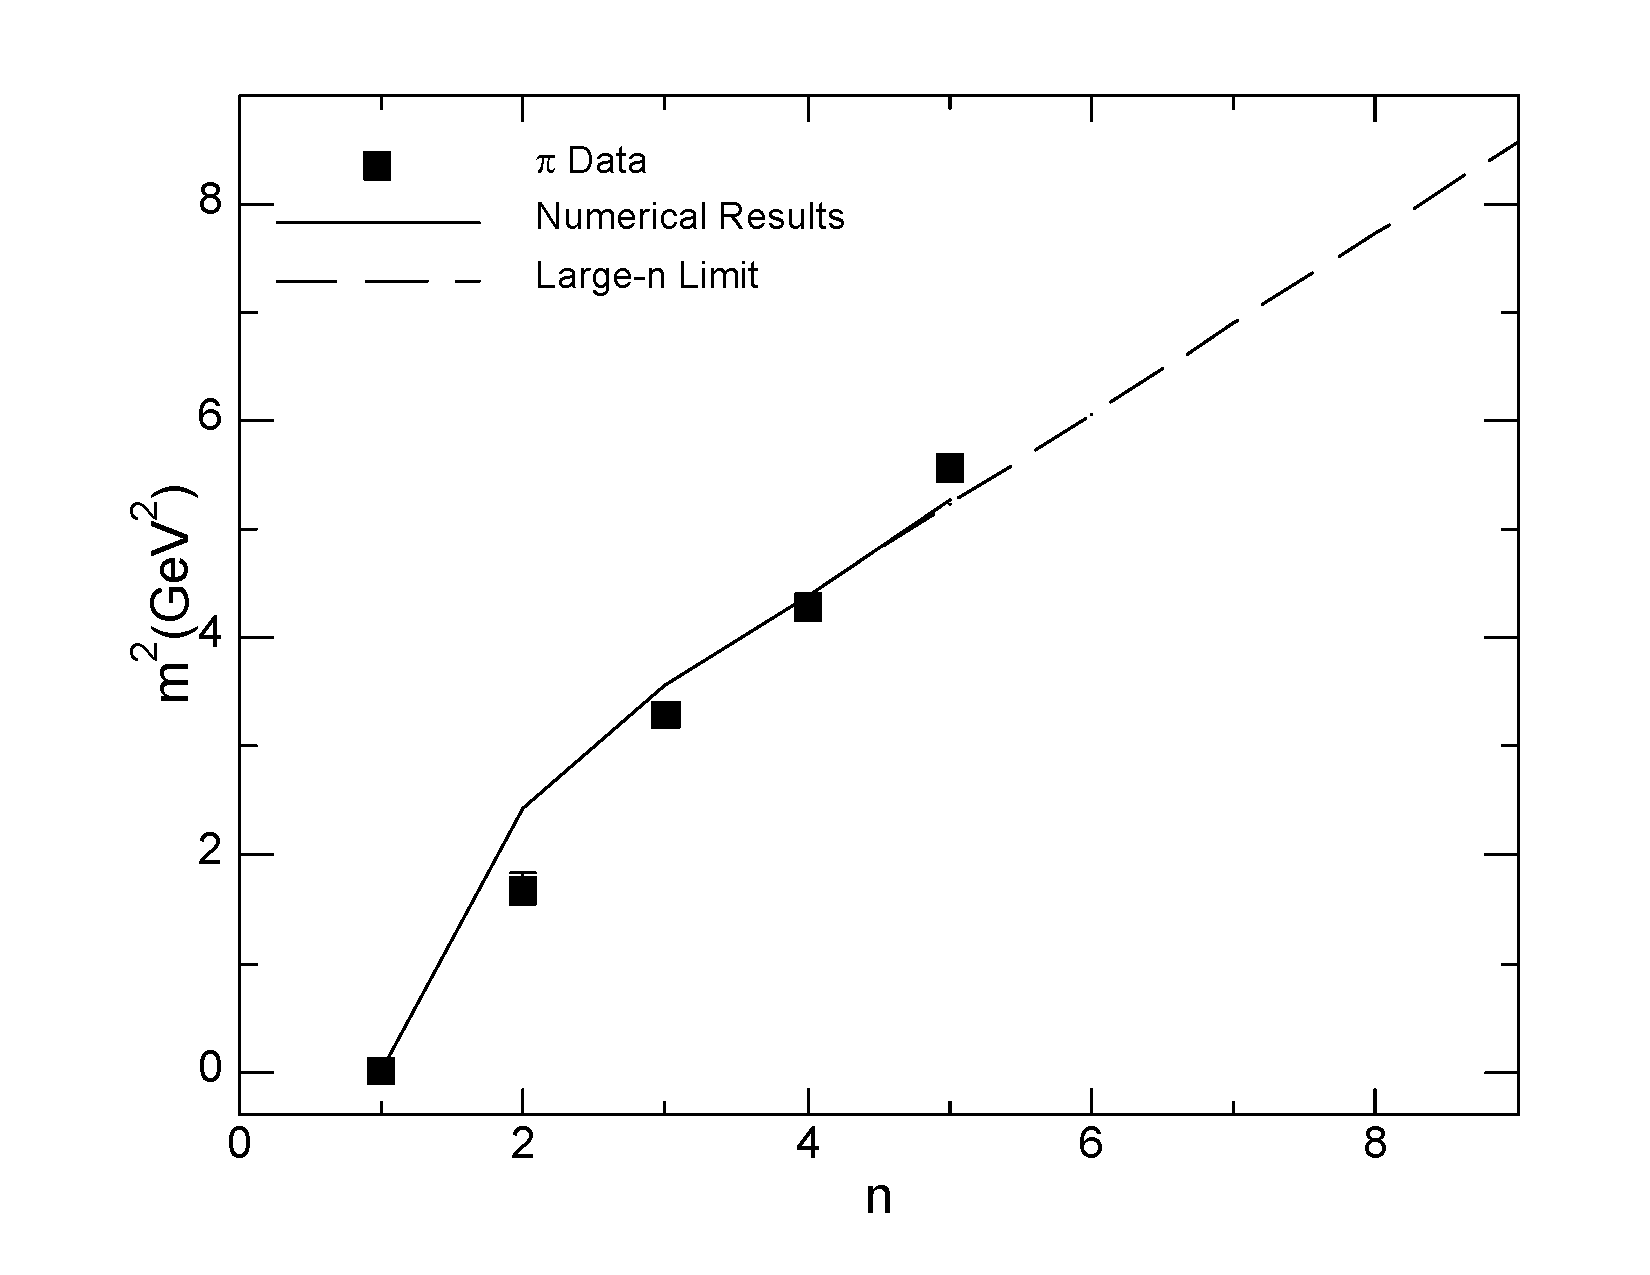
\includegraphics[width=\textwidth]{linear.pdf}
\caption{The pion mass spectrum calculated in the modified AdS/QCD model is plotted along with the experimental data \cite{PDG}. 
The eigenvalues display two important characteristics of the experimental pion spectrum: (1) light ground state and (2) a large gap between the ground state and the first excited state. 
The large-$n$ mass trajectory clearly follows our calculated eigenvalues from $n\approx 4$ when our numerical routine inadequately follows the oscillations of the higher eigenfunctions.}
\label{fig:mass}
\end{center}
\end{figure}



For large-$n$ excitations the numerical technique develops problems
with the boundary conditions. As the number of oscillations in the
eigenfunctions increase for higher $n$ modes, the routine finds eigenvalues
that are skewed to larger values. To uncover the correct asymptotic
behavior for large $n$, we take the large-$z$ limit of (\ref{equSchphi})
and (\ref{equSchpi}). As $n$ increases, the eigenfunction is largely
determined by the behavior of the effective potential at large $z$.
At large $z$, the VEV and dilaton behave as 
\ba
\chi(z) & = & (\alpha+\beta)z\equiv\Gamma\frac{z}{L}\\
\phi(z) & = & \lambda z^{2}.
\ea


To take the large-$z$ limit of the linear representation, we introduce a new dimensionless parameter, $\xi=\sqrt{\lambda}z$, and expand in $\xi$. 
In the linear representation, we find that (\ref{equSchphi}) and (\ref{equSchpi}) at large $\xi$ become 
\ba
-\pi_{k}''+\xi^{2}\pi_{k} & = & \left(\frac{\kappa\Gamma^{2}}{2\lambda}-2+\frac{m_{k}^{2}}{\lambda}\right)\pi_{k}-\frac{m_{k}^{2}\Gamma}{\lambda}\varphi_{k}\label{equpiSHO}\\
-\varphi_{k}''+\xi^{2}\varphi_{k} & = & \frac{g_{5}^{2}\Gamma}{\lambda}\left(\pi_{k}-\Gamma\varphi_{k}\right)\label{equphiSHO}
\ea
where ($'$) here indicates differentiation with respect to $\xi$.
This set of equations has the form of coupled harmonic oscillators, the equations of motion of which are 
\ba
-\varphi_{k}''+\xi^{2}\varphi_{k} & = & (2k+1)\varphi{}_{k}\label{equphiSHOG}\\
-\pi_{k}''+\xi^{2}\pi_{k} & = & (2k+1)\pi_{k}\quad\quad k=0,1,\ldots.\label{equpiSHOG}
\ea
We make the reasonable assumption that $\varphi_{k}=c_{k}\pi_{k}$, which ensures that (\ref{equpiSHO}), and (\ref{equphiSHO}) have solutions. 
Using the form of (\ref{equphiSHOG}) and (\ref{equpiSHOG}) to solve for  $m_{k}^{2}$, and making use of the fact that $\Gamma^{2}=4\lambda/\kappa$, we find 
\be
m_{k}^{2}=g_{5}^{2}\Gamma^{2}+(2k+1)\lambda.
\ee
Until now we have not made use of the fact that, in the AdS metric, $z\geq0$. 
Because of this, the eigenfunctions $\varphi_{n}$ and $\pi_{n}$ describe \textit{half} harmonic oscillators with half as many modes; therefore, we must take $k\rightarrow2k$. 
The mass eigenvalues for large $n$, where $n=k+1$, in both representations then become 
\be
m_{n}^{2}=(4n-3)\lambda+g_{5}^{2}\Gamma^{2}\quad\quad n=4,5,\ldots\label{equMass4Both}
\ee
which are also listed in Table \ref{tblmass} and plotted in Figure \ref{fig:mass}. 
Combining (\ref{equMass4Both}) and the numerical technique, we obtain all the pseudoscalar eigenvalues. 
On inspection, we find that this method should be trusted over the numerical routine for $n\geq4$.


\subsection{Gell-Mann--Oakes--Renner Relation}
\label{sub:GMOR}
The mass of the ground-state pion is related to the spontaneous breaking of chiral symmetry.
Whenever a continuous symmetry is spontaneously broken, a massless particle appears -- a result  known as Goldstone's Theorem.
The resulting particles are known as Goldstone bosons, or, if the symmetry is also broken explicitly, they are called pseudo-Goldstone bosons because they are not truly massless.
The ground-state pion is the pseudo-Goldstone boson of chiral symmetry, which is the reason for its small mass in comparison to the other meson ground states.
The Gell-Mann--Oakes--Renner relation is a formula relating the mass of the pion to the quark mass and the chiral condensate \cite{GMOR}.
The relation takes the form
\be
2m_{q}\sigma=m_{\pi}^{2}f_{\pi}^{2}\, ,
\ee
 where $f_\pi$ is known as the \emph{pion decay constant} and has dimensions of mass, $\sigma$ is the quark condensate, with dimensions of $\mathrm{mass}^3$, and $m_q$ is the average of the up and down quark masses.
 This relation is explored further and derived in Appendix \ref{app_GMOR}.

\subsubsection{The Gell-Mann--Oakes--Renner Relation in Soft-Wall AdS/QCD}

We now explore the Gell-Mann--Oakes--Renner relation in the soft-wall AdS/QCD model numerically.
Inserting the established equivalence between the exponential and linear representations, $\pi_{e}=\pi_{l}/\chi(z)$, into the pion equation of motion (\ref{equOnemid}), we obtain 
\be
\frac{g_{5}^{2}L^{2}\chi^{2}}{z^{2}}\partial_{z}\left(\frac{\pi_{l}}{\chi}\right)=m_{\pi}^{2}\partial_{z}\varphi\,.\label{eq:EOM-Modified}
\ee
 Following the method of \cite{stephanov-katz-son}, we construct a perturbative solution in $m_{\pi}$ where $\varphi(z)=A(0,z)-1$ and use the established relation
\be
f_{\pi}^{2}=-\left.L\frac{\partial_{z}A(0,z)}{g_{5}^{2}z}\right|_{z\rightarrow0.}\label{eq:fpi}
\ee
Integrating (\ref{eq:EOM-Modified}) yields 
\be
\frac{\pi(z)}{\chi(z)}=m_{\pi}^{2}\int_{0}^{z}du\,\frac{u^{3}}{\chi^{2}(u)}\frac{\partial_{z}A(0,u)}{g_{5}^{2}u}\,.
\ee
The function $u^{3}/\chi^{2}(u)$ has significant support only at small values of $u\sim\sqrt{m_{q}/\sigma}$, where we may use (\ref{eq:fpi}) to relate the derivative on $A(0,u)$ to the pion decay constant, so that 
\be
\frac{\pi_{l}}{\chi}=-\frac{m_{\pi}^{2}f_{\pi}^{2}}{2m_{q}\sigma}\,.\label{equPreGOR}
\ee
We find that letting $\pi_{l}=-\chi(z)$ solves the axial-vector field's equation of motion 
\be
e^{\Phi}\partial_{z}\left(\frac{e^{-\Phi}}{z}\partial_{z}A_{\mu}(q,z)\right)-\frac{q^{2}}{z}A_{\mu}(q,z)-\frac{g_{5}^{2}L^{2}\chi^{2}}{z^{3}}A_{\mu}(q,z)=0
\ee
 in the region of small $z$ and as $q\rightarrow0$. 
 As a result, (\ref{equPreGOR}) becomes the expected Gell-Mann--Oakes--Renner (GOR)
relation, 
\be
2m_{q}\sigma=m_{\pi}^{2}f_{\pi}^{2}\,.\label{eq:GOR}
\ee

We solve for the ground-state pseudoscalar mass, $m_{\pi}$, for
differing values of $m_{q}$ to ensure that the numerical routine
respects the Gell-Mann--Oakes--Renner relation and gives a reasonable value for $f_{\pi}$.
The results are plotted in Figure \ref{fig:GOR}. We see linear behavior
in the plot, indicating that as $m_{q}\rightarrow0$ we obtain a constant
ratio of $m_{q}/m_{\pi}^{2}$. The slope of the line in Figure \ref{fig:GOR}
suggests $f_{\pi}=90$ MeV, a result consistent with the input parameters
as described in \cite{gherghetta-kelley}.

\begin{figure}[htb]
\center{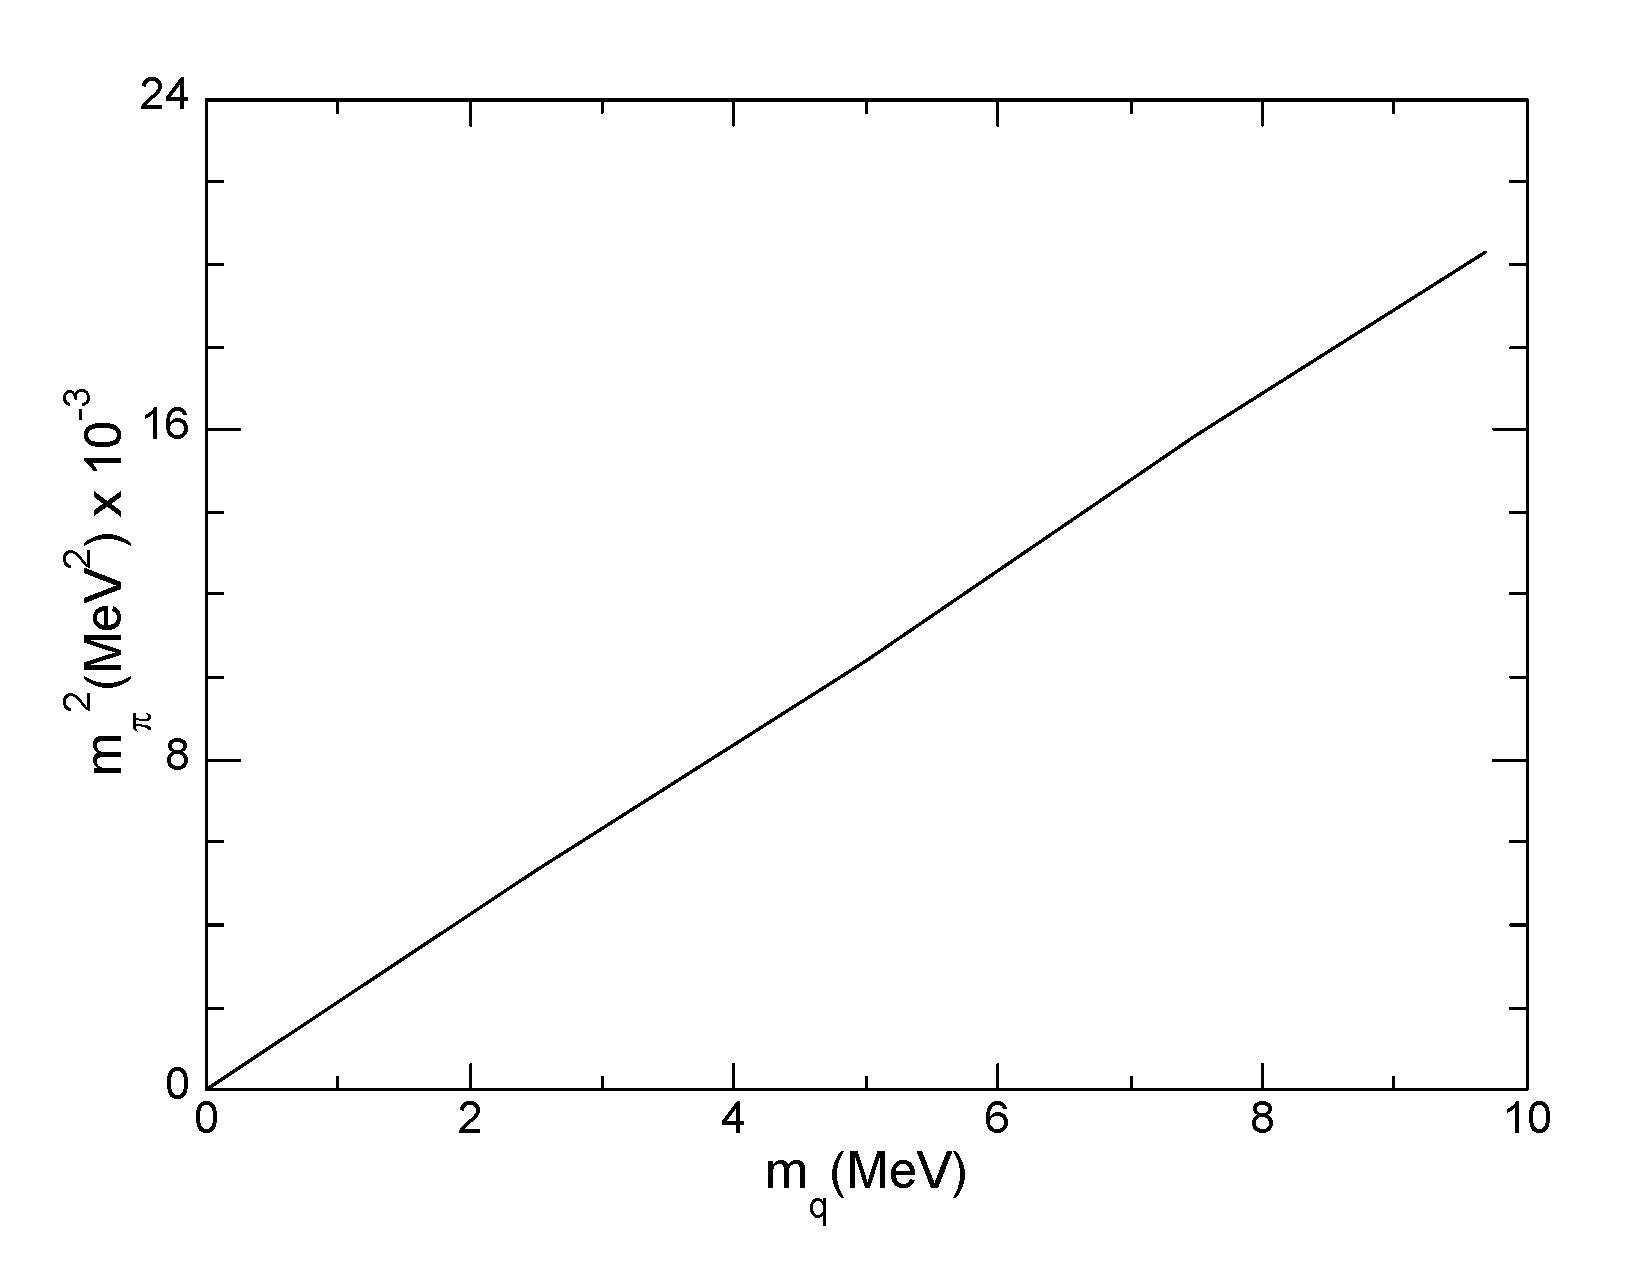
\includegraphics[width=\textwidth]{quarkvspion.pdf}}
\caption{Plot of $m_{\pi}^{2}$ vs $m_{q}$ yields a straight line from which the pion decay constant $f_{\pi}$ is calculated using (\ref{eq:GOR}).}
\label{fig:GOR}
\end{figure}

\section{Summary}
In this chapter, we discussed the metric structure and field content of a soft-wall AdS/QCD model. 
We illustrated the field content of the simplest such model that describes light mesons and their spectra.
We introduced the vacuum expectation value of the scalar field, which is related to the chiral symmetry breaking of the theory.
The behavior of this chiral condensate was derived, and we discussed the shortcomings apparent in the simplest soft-wall models.
We then derived the equations of motion for the scalar, vector, and axial-vector mesons.

We also developed a modified soft-wall model that allows for the correct form of chiral symmetry breaking.
In this model, we discussed the derivation of the pseudoscalar equations of motion, and the equivalence between the two common representations of the pseudoscalar field.
Finally, we calculated the Gell-Mann--Oakes--Renner relation in the linear representation, showing that it is equivalent to that derived in the exponential representation.
The Gell-Mann--Oakes--Renner relation is confirmed numerically in this model, and the calculated value of $f_\pi$ is in good agreement with the accepted value.